\documentclass{cshwk}

\title{Principles of Database Systems\\Assignment \#3 - Structured Query Language 1}

\begin{document}
\maketitle

\section{Execute the SQL in Slides}

\subsection{Preparation}

\subsubsection{Table Creation}

\begin{lstlisting}

CREATE TABLE Movies (
    title       CHAR(100),
    year        INT,
    length      INT,
    genre       CHAR(10),
    studioName  CHAR(30),
    producerC   INT,
    PRIMARY KEY (title, year)
);

\easyfigure{hw4-1.png}{Table Creation Results}{fig:table-creation}

\end{lstlisting}

The execute results is shown in Figure \ref{fig:table-creation}.
\begin{figure}[htbp]
    \centering
    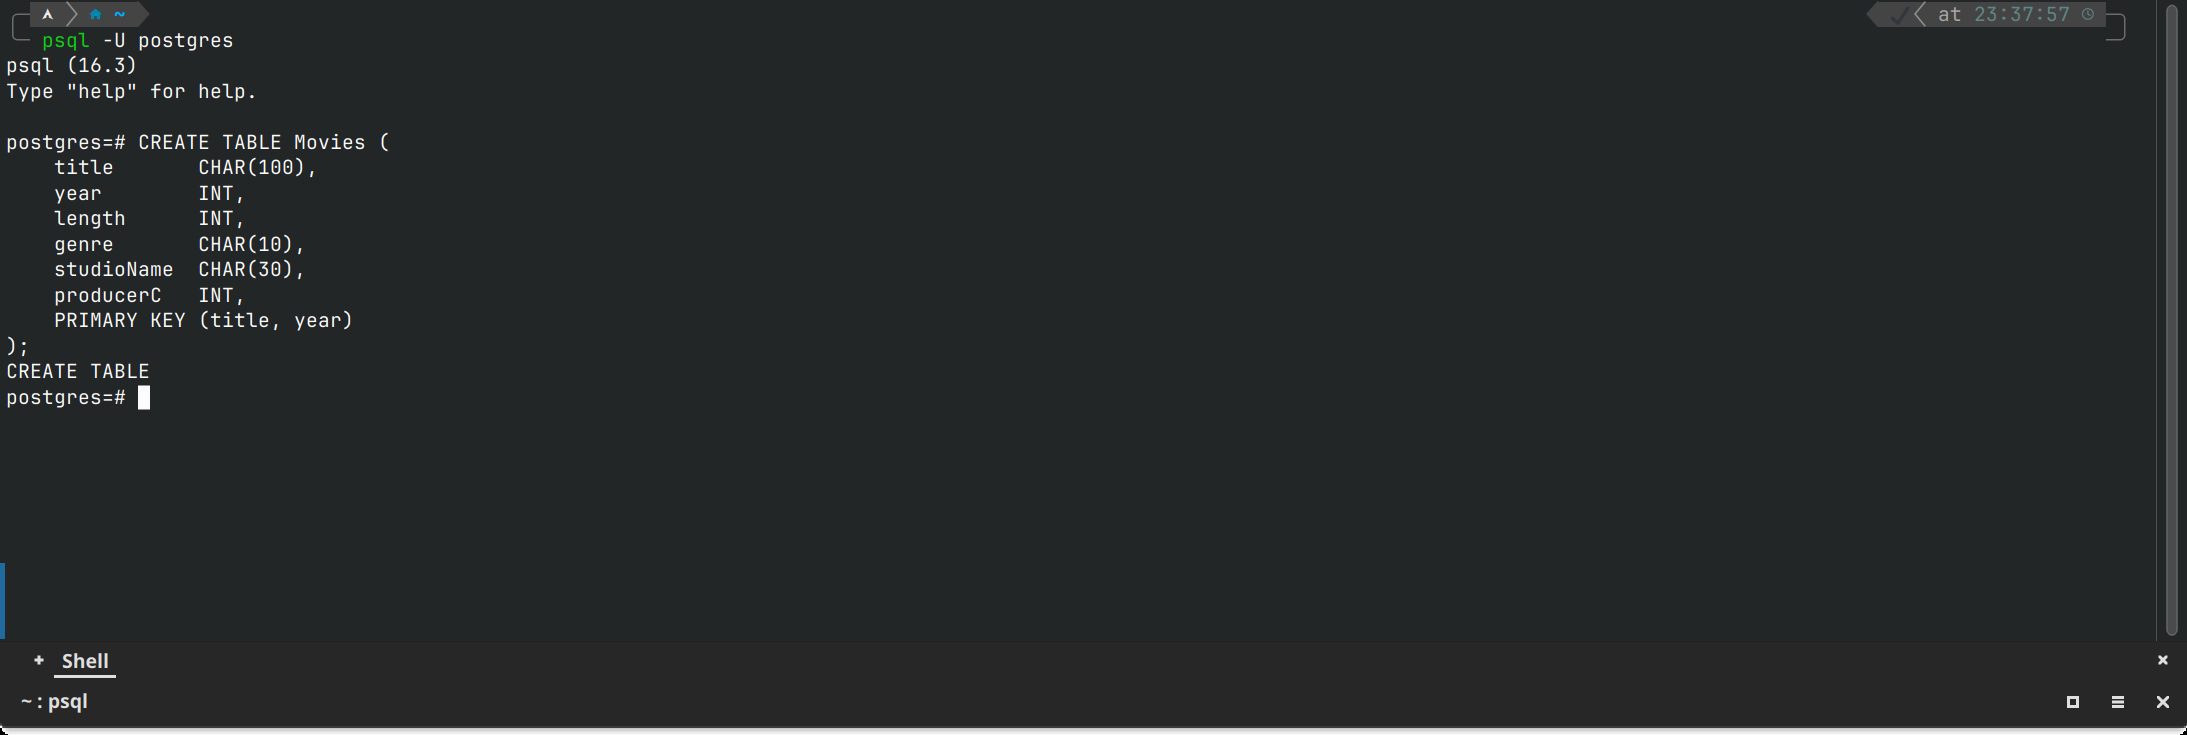
\includegraphics[width=0.8\textwidth]{hw4-1.png}
    \caption{Table Creation Results}
    \label{fig:table-creation}
\end{figure}

\subsubsection{Sample Data in \texttt{Movies} Table}

\begin{lstlisting}
INSERT INTO movies VALUES ('Logan''s run', 1976, NULL, 'sciFi', 'MGM', 123);
INSERT INTO movies VALUES ('Star Wars', 1977, 124, 'sciFi', 'Fox', 555);
INSERT INTO movies VALUES ('Empire Strikes Back', 1980, 111, 'fantasy', 'Fox', 555);
INSERT INTO movies VALUES ('Star Trek', 1979, 132, 'sciFi', 'Paramount', 345);
INSERT INTO movies VALUES ('Star Trek: Nemesis', 2002, 116, 'sciFi', 'Paramount', 345);
INSERT INTO movies VALUES ('Terms of Endearment', 1983, 132, 'romance', 'MGM', 123);
INSERT INTO movies VALUES ('The Usual Suspects', 1995, 106, 'crime', 'MGM', 456);
INSERT INTO movies VALUES ('Gone With the Wind', 1938, 238, 'drama', 'MGM', 123);
INSERT INTO movies VALUES ('Wayne''s World', 1992, 95, 'comedy', 'Paramount', 123);
INSERT INTO movies VALUES ('King Kong', 2005, 187, 'drama', 'Universal', 789);
INSERT INTO movies VALUES ('King Kong', 1976, 134, 'drama', 'Paramount', 666);
INSERT INTO movies VALUES ('King Kong', 1933, 100, 'drama', 'Universal', 345);
INSERT INTO movies VALUES ('Pretty Woman', 1990, 119, 'comedy', 'Disney', 999);
\end{lstlisting}

The execute results is shown in Figure \ref{fig:sample-data}.
\begin{figure}[htbp]
    \centering
    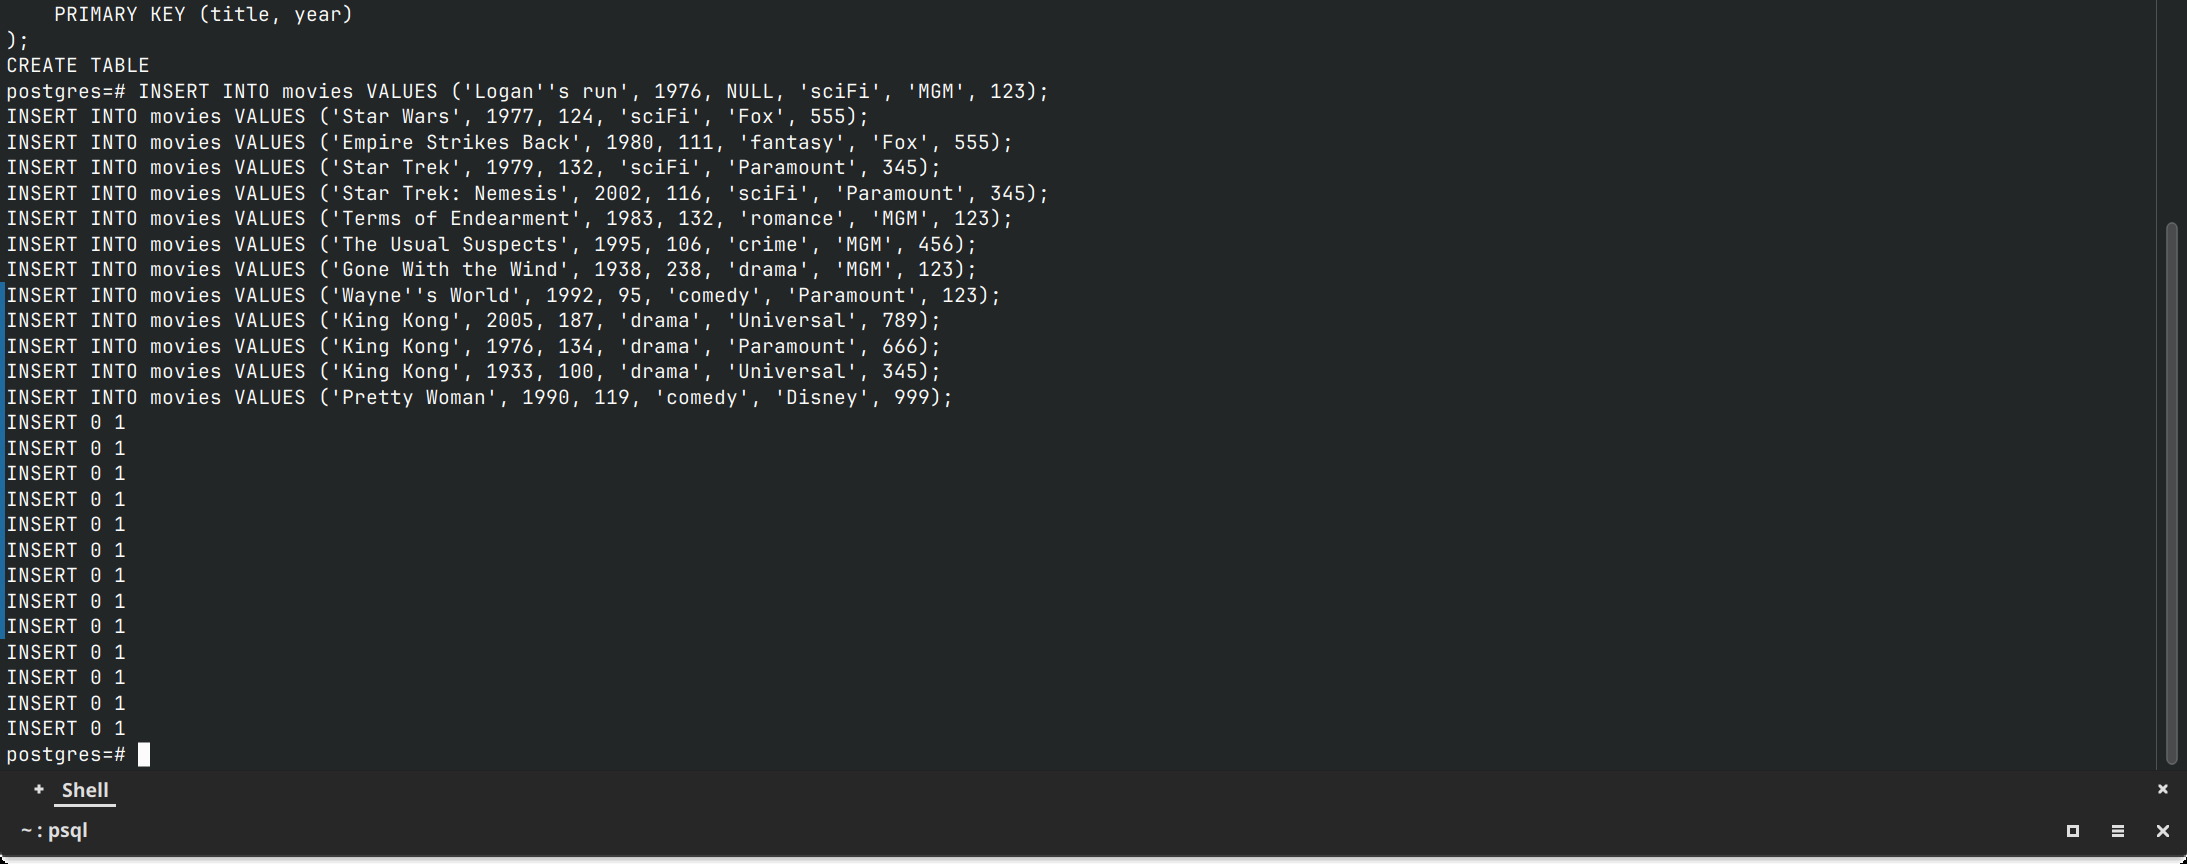
\includegraphics[width=0.8\textwidth]{hw4-2.png}
    \caption{Sample Data Insertion Results}
    \label{fig:sample-data}
\end{figure}

\subsection{Queries}

\subsubsection{Simple Query}

\begin{lstlisting}
SELECT * FROM movies where studioname='Disney' AND year=1990;
SELECT title, length FROM movies where studioname='Disney' AND year=1990;
SELECT title AS name, length AS duration FROM movies where studioname='Disney' AND year=1990;
SELECT title AS name, length*0.016667 as lengthInHours FROM movies WHERE studioname='Disney' AND year=1990;
SELECT title AS name, length*0.016667 as lengthInHours, 'hrs' as inHours FROM movies WHERE studioname='Disney' AND year=1990;
\end{lstlisting}

The execute results is shown in Figure \ref{fig:simple-query}.
\begin{figure}[htbp]
    \centering
    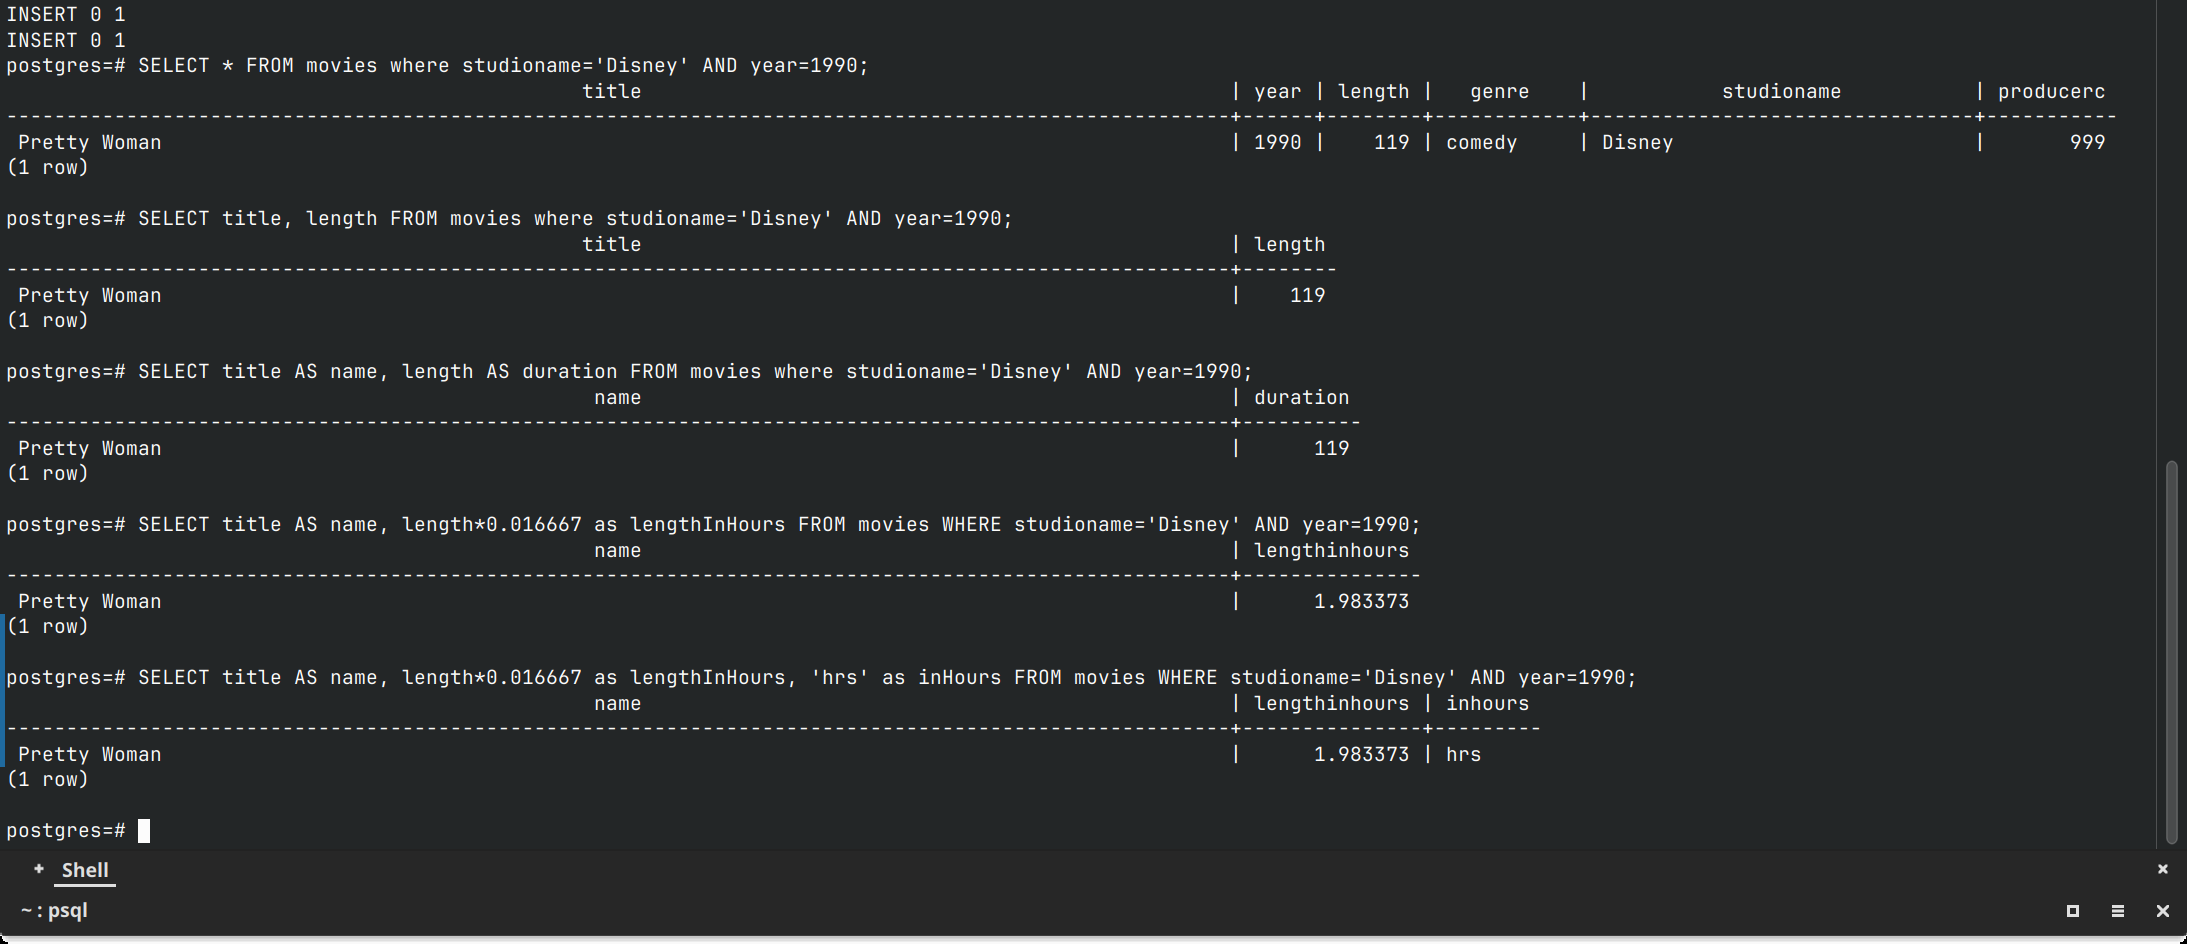
\includegraphics[width=0.9\textwidth]{hw4-3.png}
    \caption{Simple Query Results}
    \label{fig:simple-query}
\end{figure}

\subsubsection{Query with Complex WHERE}

\begin{lstlisting}
SELECT title FROM movies WHERE (year > 1970 OR  length < 90) AND studioname='MGM';
SELECT title FROM movies WHERE year between 1970 and 2000;
SELECT title FROM movies WHERE title LIKE '%Star W__s%';
SELECT title FROM movies WHERE title LIKE '%''s%';
\end{lstlisting}

The execute results is shown in Figure \ref{fig:complex-where}.
\begin{figure}[htbp]
    \centering
    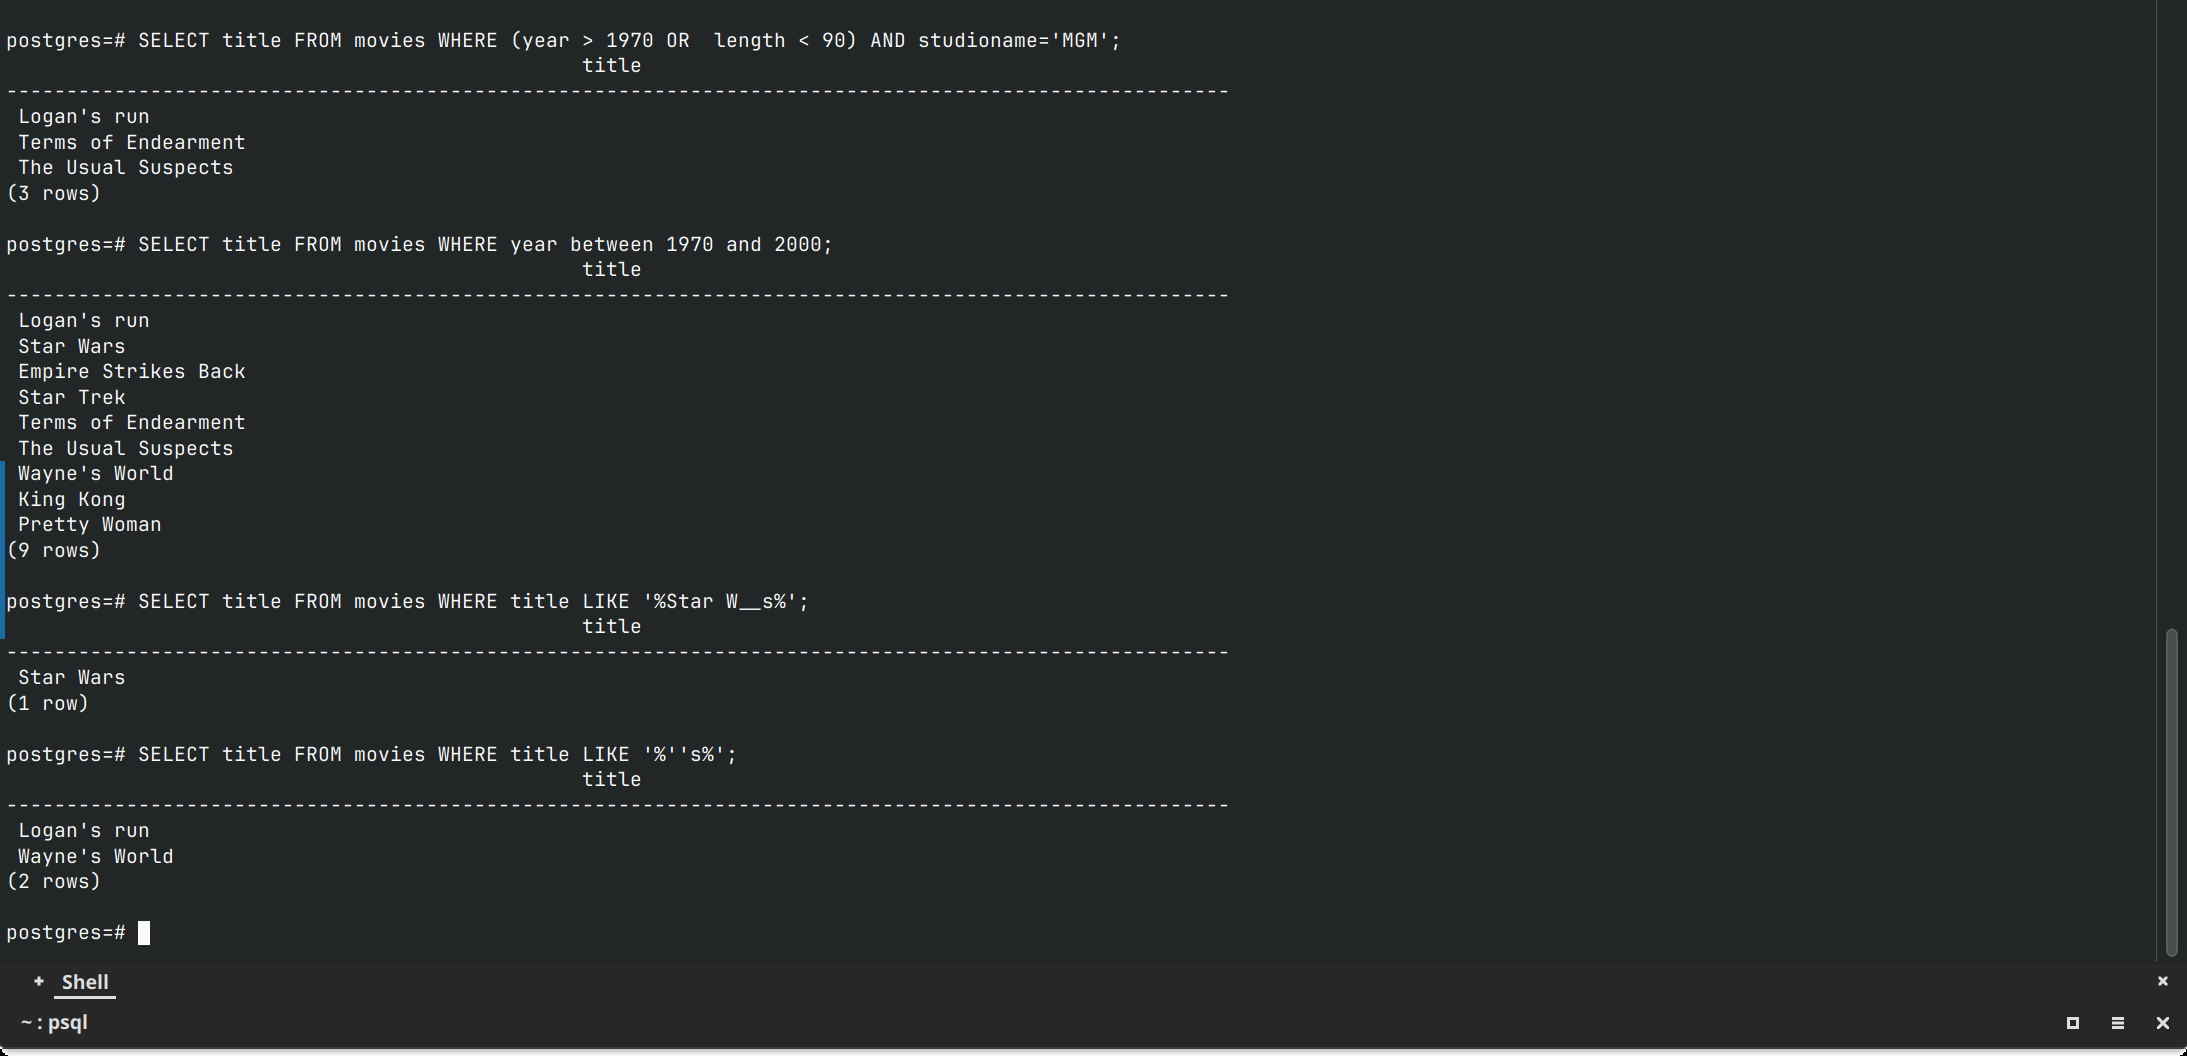
\includegraphics[width=0.9\textwidth]{hw4-4.png}
    \caption{Query with Complex WHERE Results}
    \label{fig:complex-where}
\end{figure}

\subsubsection{Query with \texttt{NULL} Values}

\begin{lstlisting}
INSERT INTO movies VALUES ('ABC', 1976, NULL, 'sciFi', 'MGM', NULL);

SELECT title, movies.length=3 FROM Movies;
SELECT title, movies.length+3 FROM Movies;
\end{lstlisting}

The execute results is shown in Figure \ref{fig:null-values}.
\begin{figure}[htbp]
    \centering
    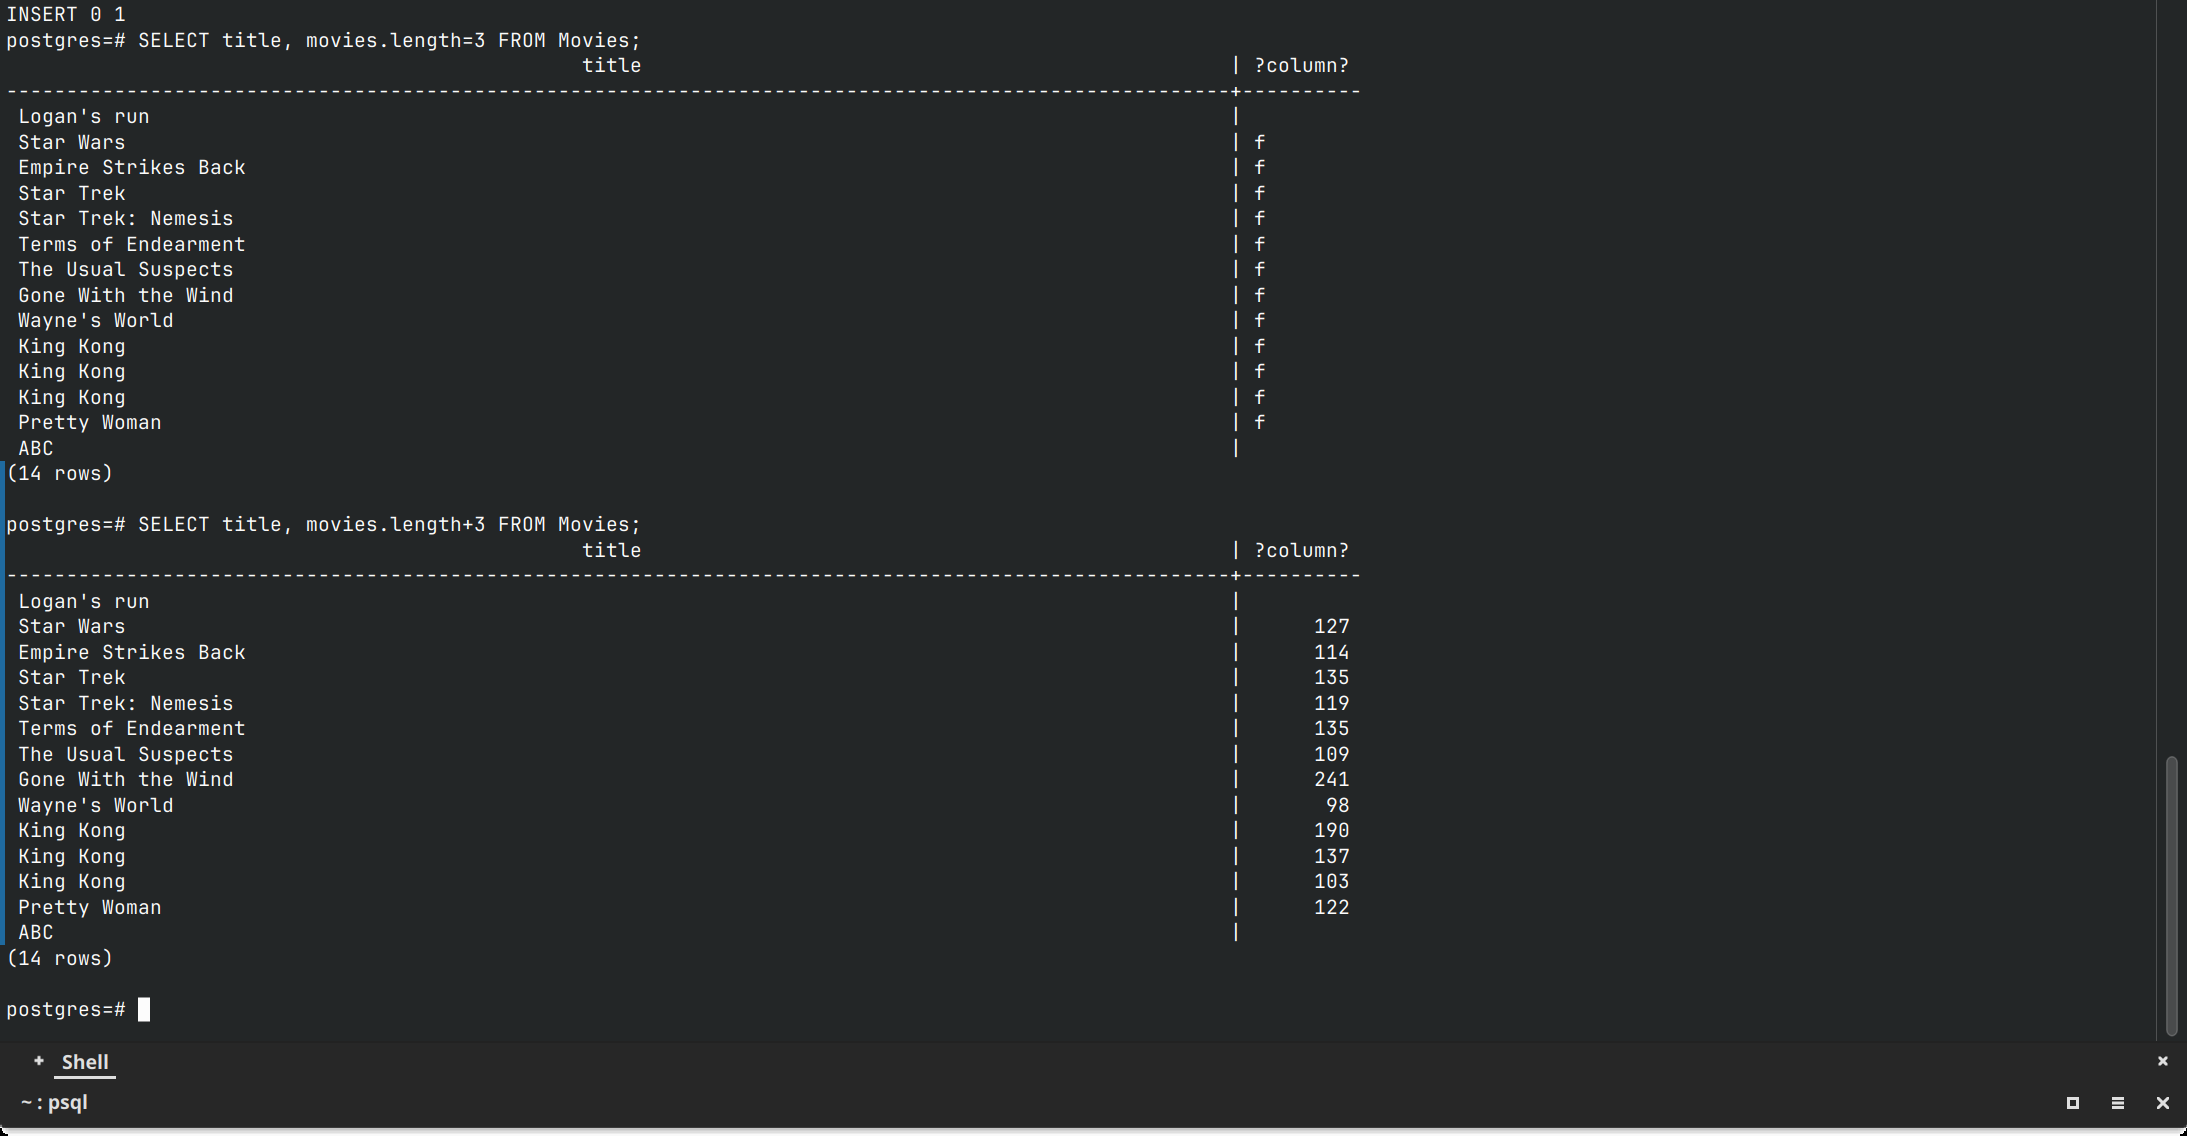
\includegraphics[width=0.9\textwidth]{hw4-5.png}
    \caption{Query with \texttt{NULL} Values Results}
    \label{fig:null-values}
\end{figure}

\begin{lstlisting}
SELECT * FROM movies WHERE movies.length==NULL;
SELECT * FROM movies WHERE movies.length!=NULL;
SELECT * FROM movies WHERE movies.length is NULL;
SELECT * FROM movies WHERE movies.length is not NULL;
\end{lstlisting}

The execute results is shown in Figure \ref{fig:null-values-2}.
\begin{figure}[htbp]
    \centering
    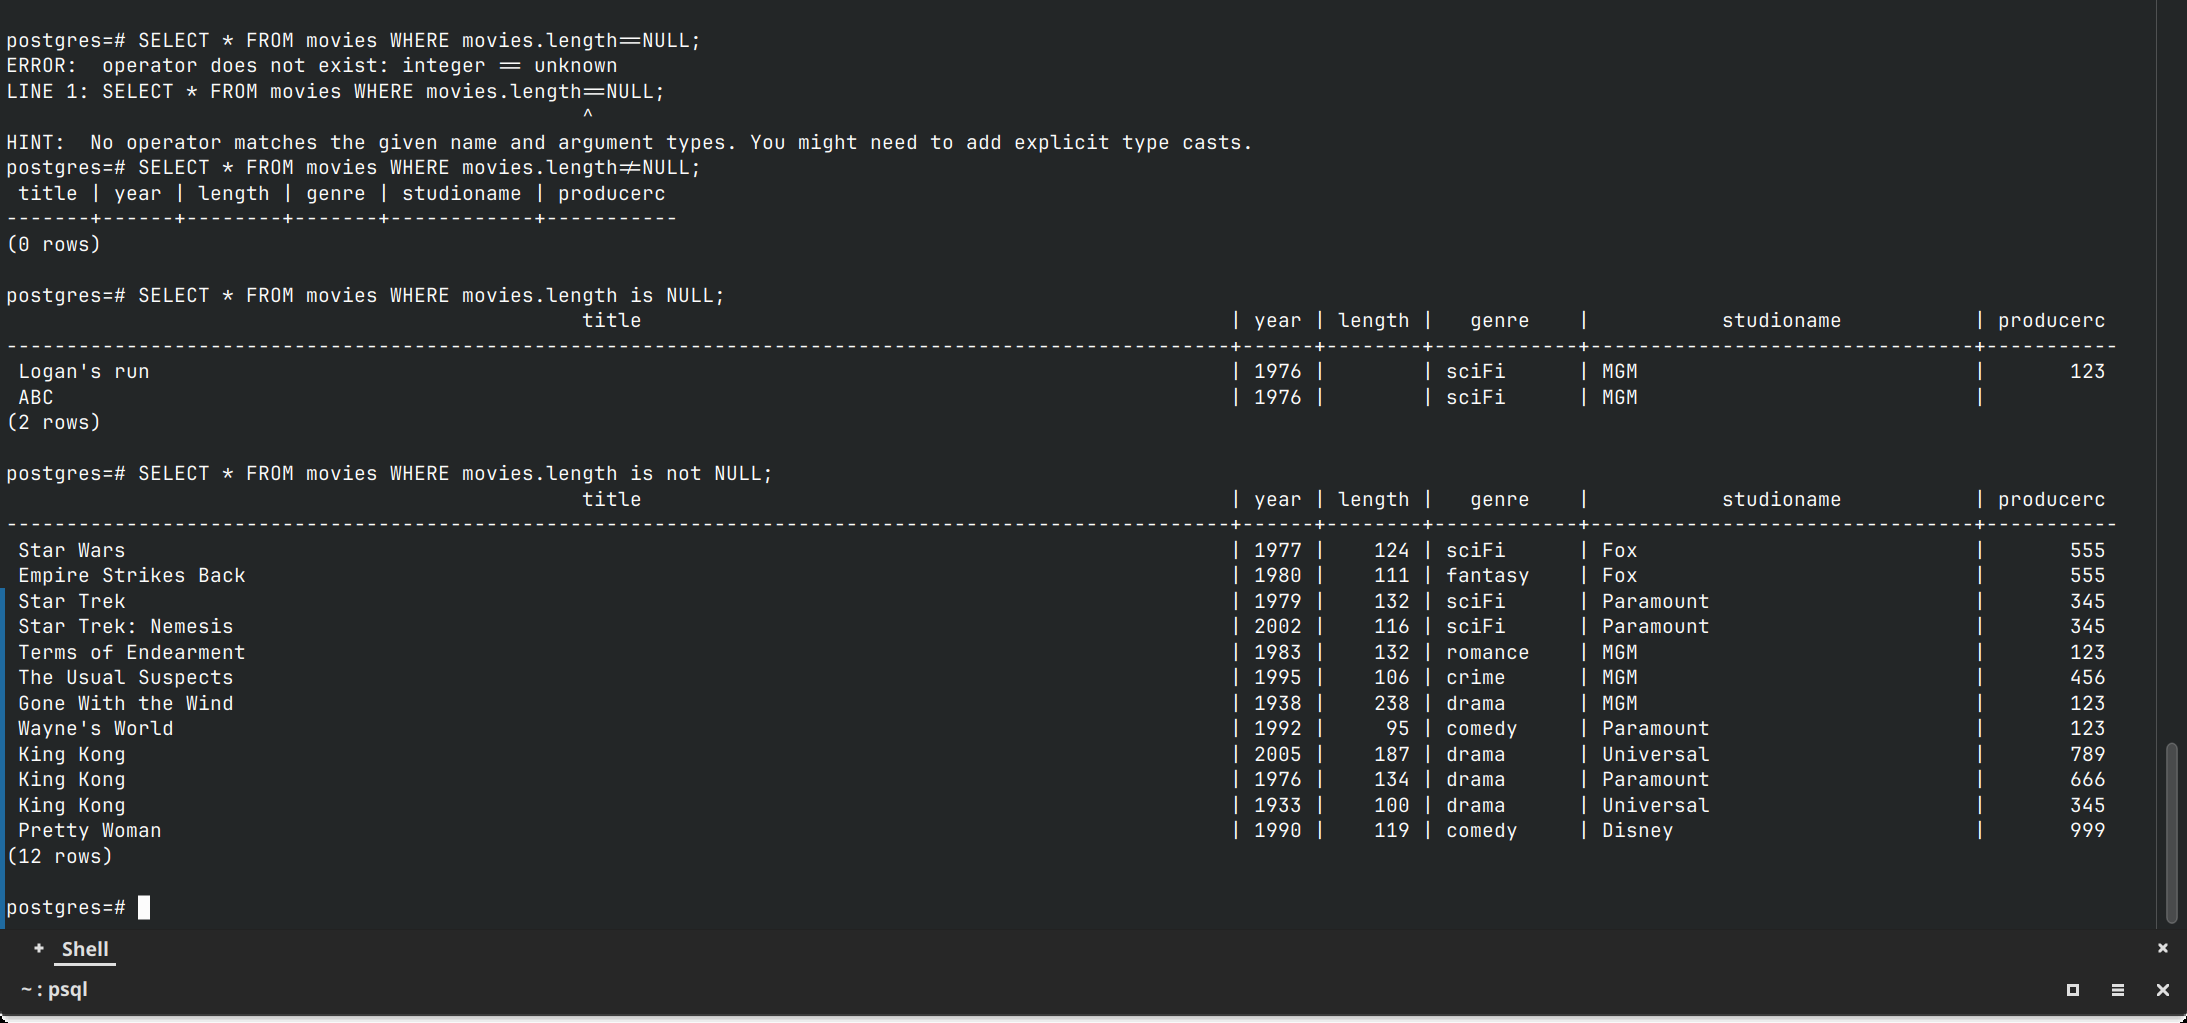
\includegraphics[width=0.9\textwidth]{hw4-6.png}
    \caption{Query with \texttt{NULL} Values Results}
    \label{fig:null-values-2}
\end{figure}

\begin{lstlisting}
SELECT * FROM movies WHERE length<=120 OR length>120;
\end{lstlisting}

The execute results is shown in Figure \ref{fig:null-values-3}.
\begin{figure}[htbp]
    \centering
    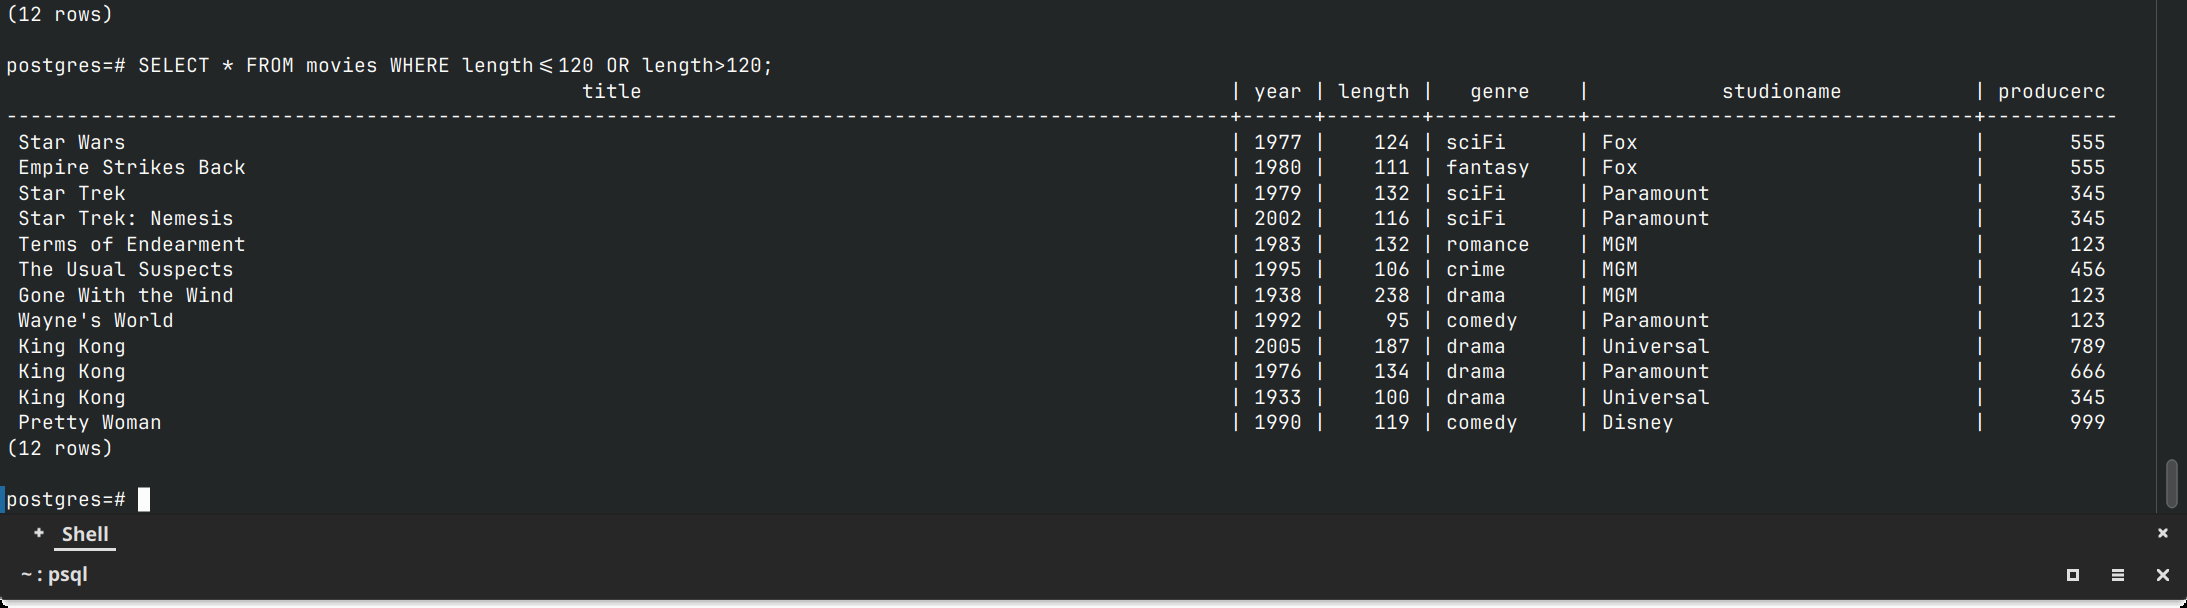
\includegraphics[width=0.9\textwidth]{hw4-7.png}
    \caption{Query with \texttt{NULL} Values Results}
    \label{fig:null-values-3}
\end{figure}


\subsubsection{Query with Ordering}

\begin{lstlisting}
SELECT * FROM movies ORDER BY length, title;
SELECT * FROM movies ORDER BY length+year DESC;
\end{lstlisting}

The execute results is shown in Figure \ref{fig:ordering}.
\begin{figure}[htbp]
    \centering
    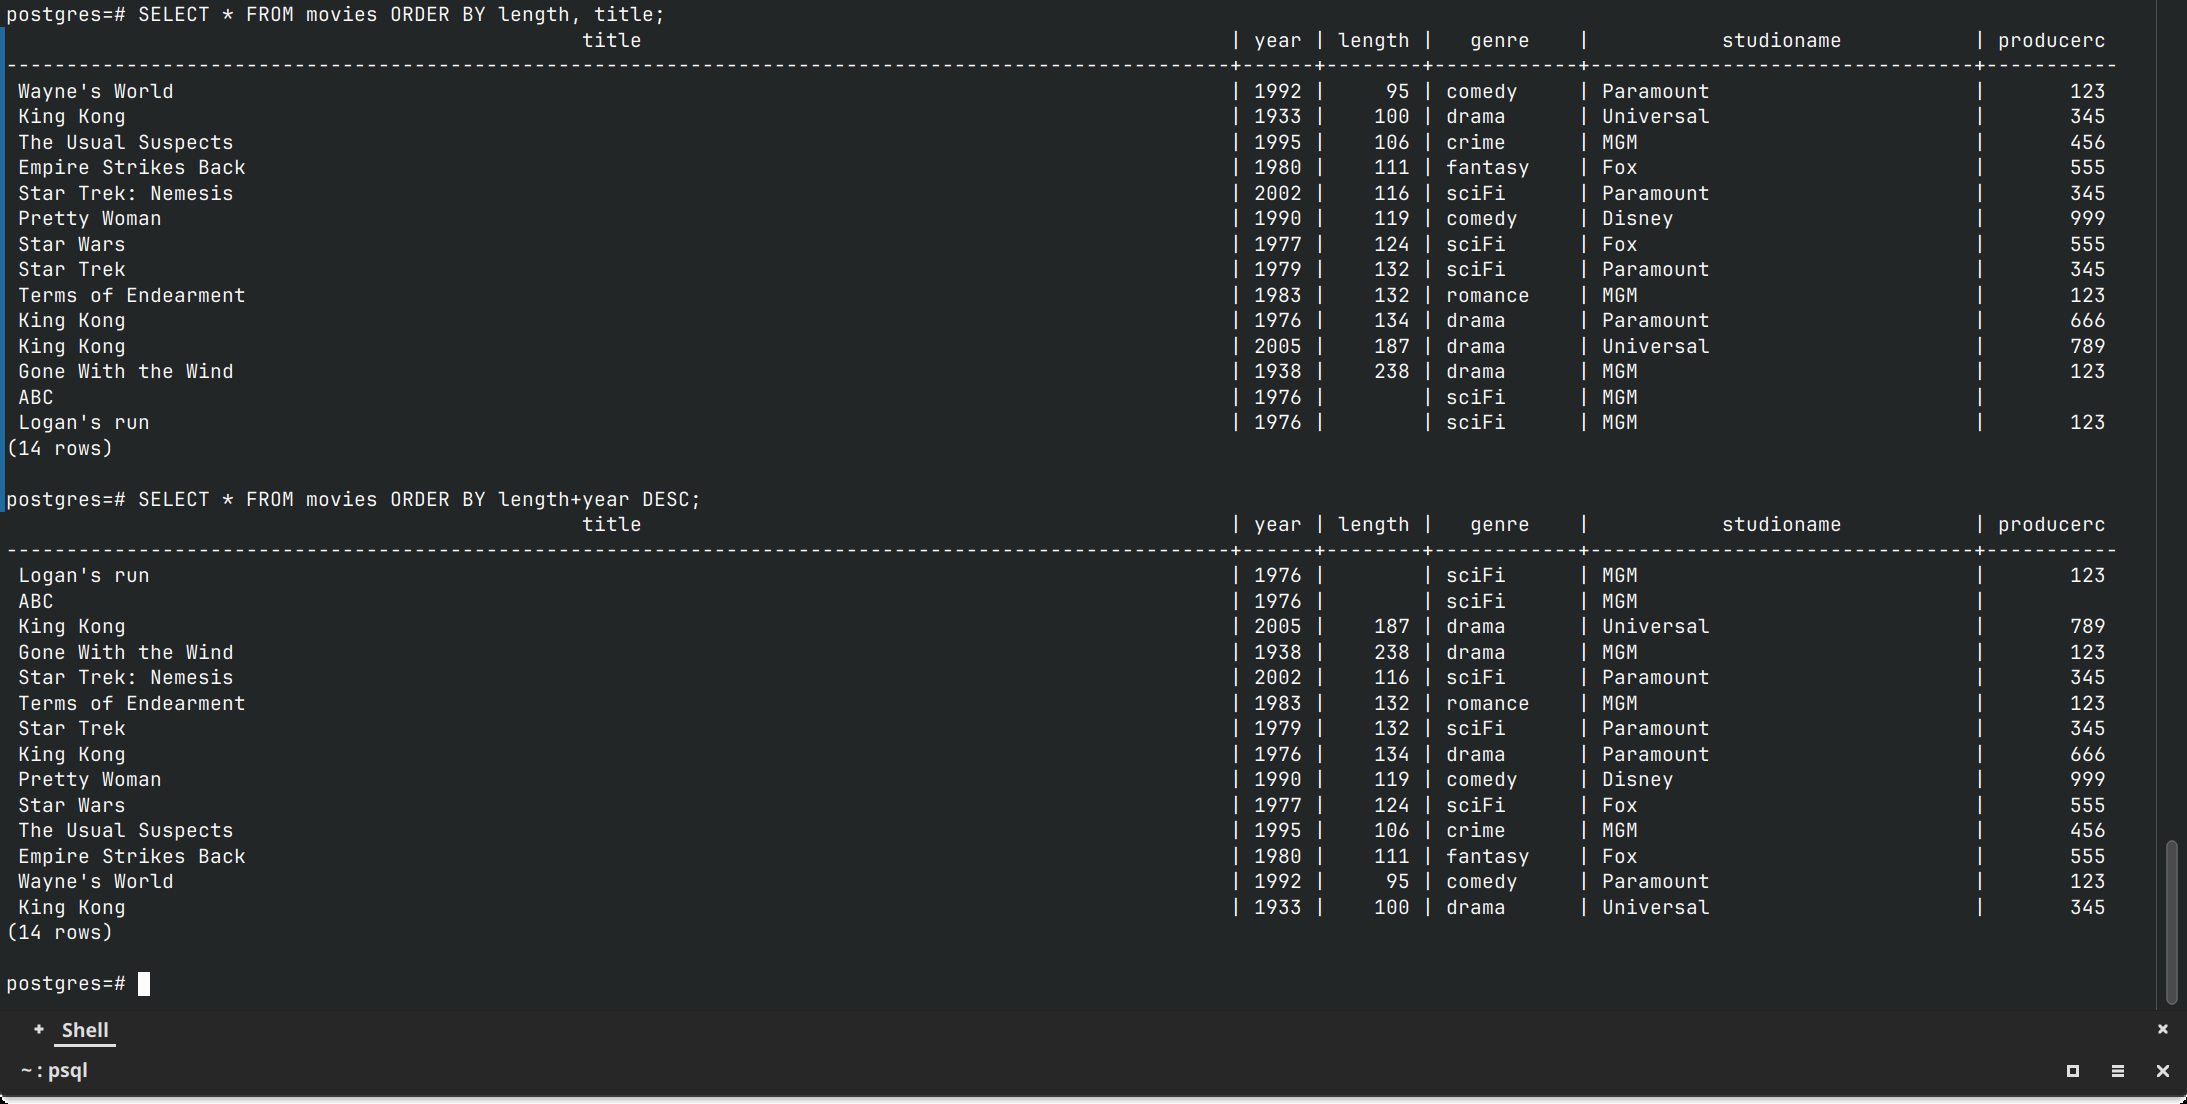
\includegraphics[width=0.9\textwidth]{hw4-8.png}
    \caption{Query with Ordering Results}
    \label{fig:ordering}
\end{figure}

\subsection{Queries on More Than One Table}

\subsubsection{Preparation}

\begin{lstlisting}
drop table movies;

CREATE TABLE movieexec (
    name        CHAR(30),
    address     VARCHAR(255),
    cert        INT,
    networth    INT
);

CREATE TABLE moviestar (
    name        CHAR(30),
    address     VARCHAR(255),
    gender      CHAR(1),
    birthdate   DATE
);

CREATE TABLE starsin (
    movietitle  CHAR(100),
    movieyear   INT,
    starname    CHAR(30)
);

CREATE TABLE Movies (
    title       CHAR(100),
    year        INT,
    length      INT,
    genre       CHAR(10),
    studioName  CHAR(30),
    producerC   INT,
    PRIMARY KEY (title, year)
);
\end{lstlisting}

the execute results is shown in Figure \ref{fig:more-than-one-table}.
\begin{figure}[htbp]
    \centering
    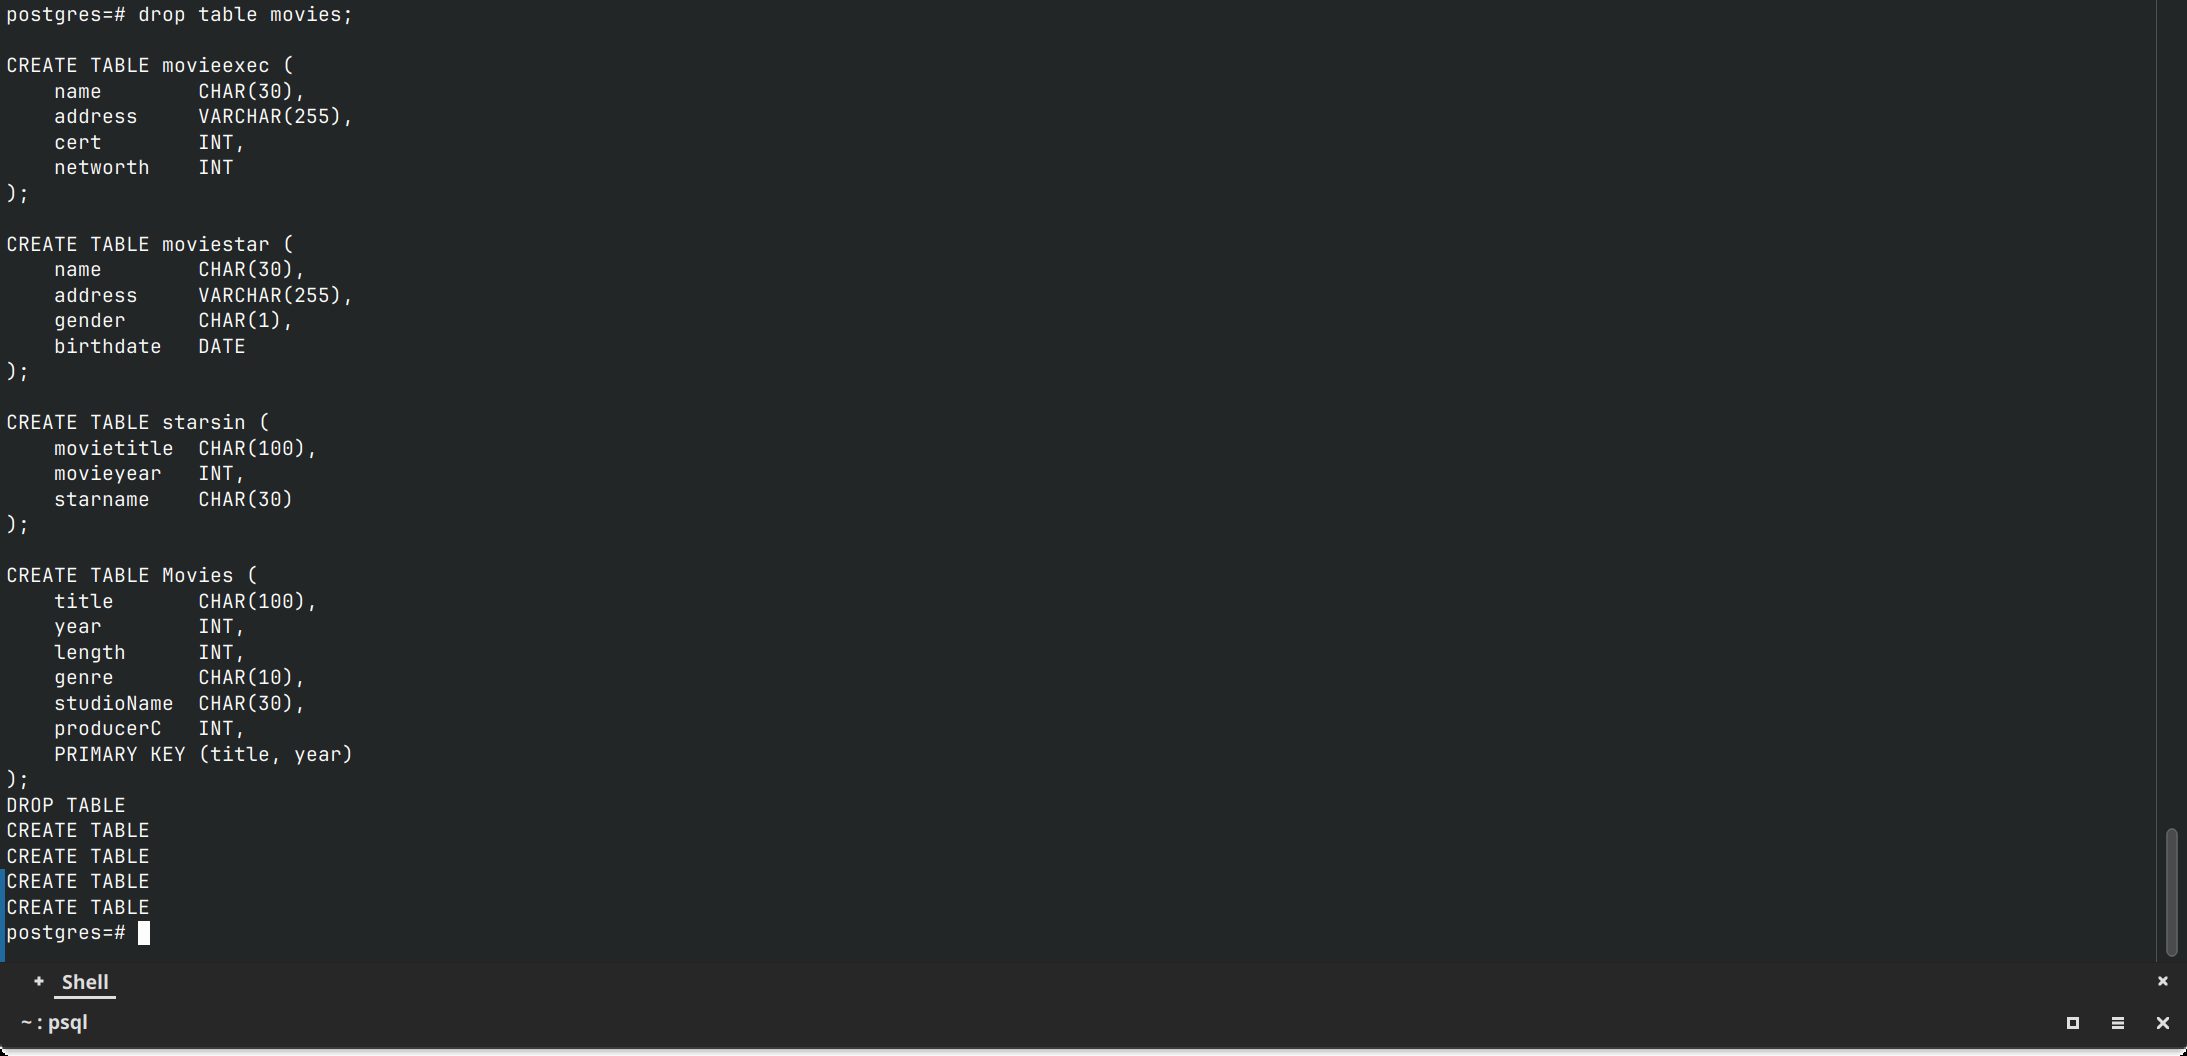
\includegraphics[width=0.9\textwidth]{hw4-9.png}
    \caption{Queries on More Than One Table Results}
    \label{fig:more-than-one-table}
\end{figure}

\subsubsection{Example Data}
\begin{lstlisting}
-- table movies
INSERT INTO movies VALUES ('Logan''s run', 1976, NULL, 'sciFi', 'MGM', 123);
INSERT INTO movies VALUES ('Star Wars', 1977, 124, 'sciFi', 'Fox', 555);
INSERT INTO movies VALUES ('Empire Strikes Back', 1980, 111, 'fantasy', 'Fox', 555);
INSERT INTO movies VALUES ('Star Trek', 1979, 132, 'sciFi', 'Paramount', 345);
INSERT INTO movies VALUES ('Star Trek: Nemesis', 2002, 116, 'sciFi', 'Paramount', 345);
INSERT INTO movies VALUES ('Terms of Endearment', 1983, 132, 'romance', 'MGM', 123);
INSERT INTO movies VALUES ('The Usual Suspects', 1995, 106, 'crime', 'MGM', 456);
INSERT INTO movies VALUES ('Gone With the Wind', 1938, 238, 'drama', 'MGM', 123);
INSERT INTO movies VALUES ('Wayne''s World', 1992, 95, 'comedy', 'Paramount', 123);
INSERT INTO movies VALUES ('King Kong', 2005, 187, 'drama', 'Universal', 789);
INSERT INTO movies VALUES ('King Kong', 1976, 134, 'drama', 'Paramount', 666);
INSERT INTO movies VALUES ('King Kong', 1933, 100, 'drama', 'Universal', 345);
INSERT INTO movies VALUES ('Pretty Woman', 1990, 119, 'comedy', 'Disney', 999);

-- table movieexec
INSERT INTO movieexec VALUES ('George Lucas', 'Oak Rd.', 555, 200000000);
INSERT INTO movieexec VALUES ('Ted Turner', 'Turner Av.', 333, 125000000);
INSERT INTO movieexec VALUES ('Stephen Spielberg', '123 ET road', 222, 100000000);
INSERT INTO movieexec VALUES ('Merv Griffin', 'Riot Rd.', 199, 112000000);
INSERT INTO movieexec VALUES ('Calvin Coolidge', 'Fast Lane', 123, 20000000);
INSERT INTO movieexec VALUES ('Garry Marshall', 'First Street', 999, 50000000);
INSERT INTO movieexec VALUES ('J.J. Abrams', 'High Road', 345, 45000000);
INSERT INTO movieexec VALUES ('Bryan Singer', 'Downtown', 456, 70000000);
INSERT INTO movieexec VALUES ('George Roy Hill', 'Baldwin Av.', 789, 20000000);
INSERT INTO movieexec VALUES ('Dino De Laurentiis', 'Beverly Hills', 666, 120000000);
INSERT INTO movieexec VALUES ('AAA', 'Beverly Hills', 666, 120000000);

-- table moviestar
INSERT INTO moviestar VALUES ('Jane Fonda', 'Turner Av.', 'F', '1977-07-07');
INSERT INTO moviestar VALUES ('Alec Baldwin', 'Baldwin Av.', 'M', '1977-06-07');
INSERT INTO moviestar VALUES ('Kim Basinger', 'Baldwin Av.', 'F', '1979-05-07');
INSERT INTO moviestar VALUES ('Harrison Ford', 'Beverly Hills', 'M', '1977-07-07');
INSERT INTO moviestar VALUES ('Carrie Fisher', '123 Maple St.', 'F', '1999-09-09');
INSERT INTO moviestar VALUES ('Mark Hamill', '456 Oak Rd.', 'M', '1988-08-08');
INSERT INTO moviestar VALUES ('Debra Winger', 'A way', 'F', '1978-05-06');
INSERT INTO moviestar VALUES ('Jack Nicholson', 'X path', 'M', '1949-05-05');
INSERT INTO moviestar VALUES ('Kevin Spacey', 'New York Av.', 'F', '1937-12-21');
INSERT INTO moviestar VALUES ('AAA', 'New York Av.', 'F', '1937-12-21');

-- table starsin
INSERT INTO starsin VALUES ('Star Wars', 1977, 'Carrie Fisher');
INSERT INTO starsin VALUES ('Star Wars', 1977, 'Mark Hamill');
INSERT INTO starsin VALUES ('Star Wars', 1977, 'Harrison Ford');
INSERT INTO starsin VALUES ('Empire Strikes Back', 1980, 'Harrison Ford');
INSERT INTO starsin VALUES ('The Usual Suspects', 1995, 'Kevin Spacey');
INSERT INTO starsin VALUES ('Terms of Endearment', 1983, 'Debra Winger');
INSERT INTO starsin VALUES ('Terms of Endearment', 1983, 'Jack Nicholson');
\end{lstlisting}

the execute results is shown in Figure \ref{fig:more-than-one-table-2}.
\begin{figure}[htbp]
    \centering
    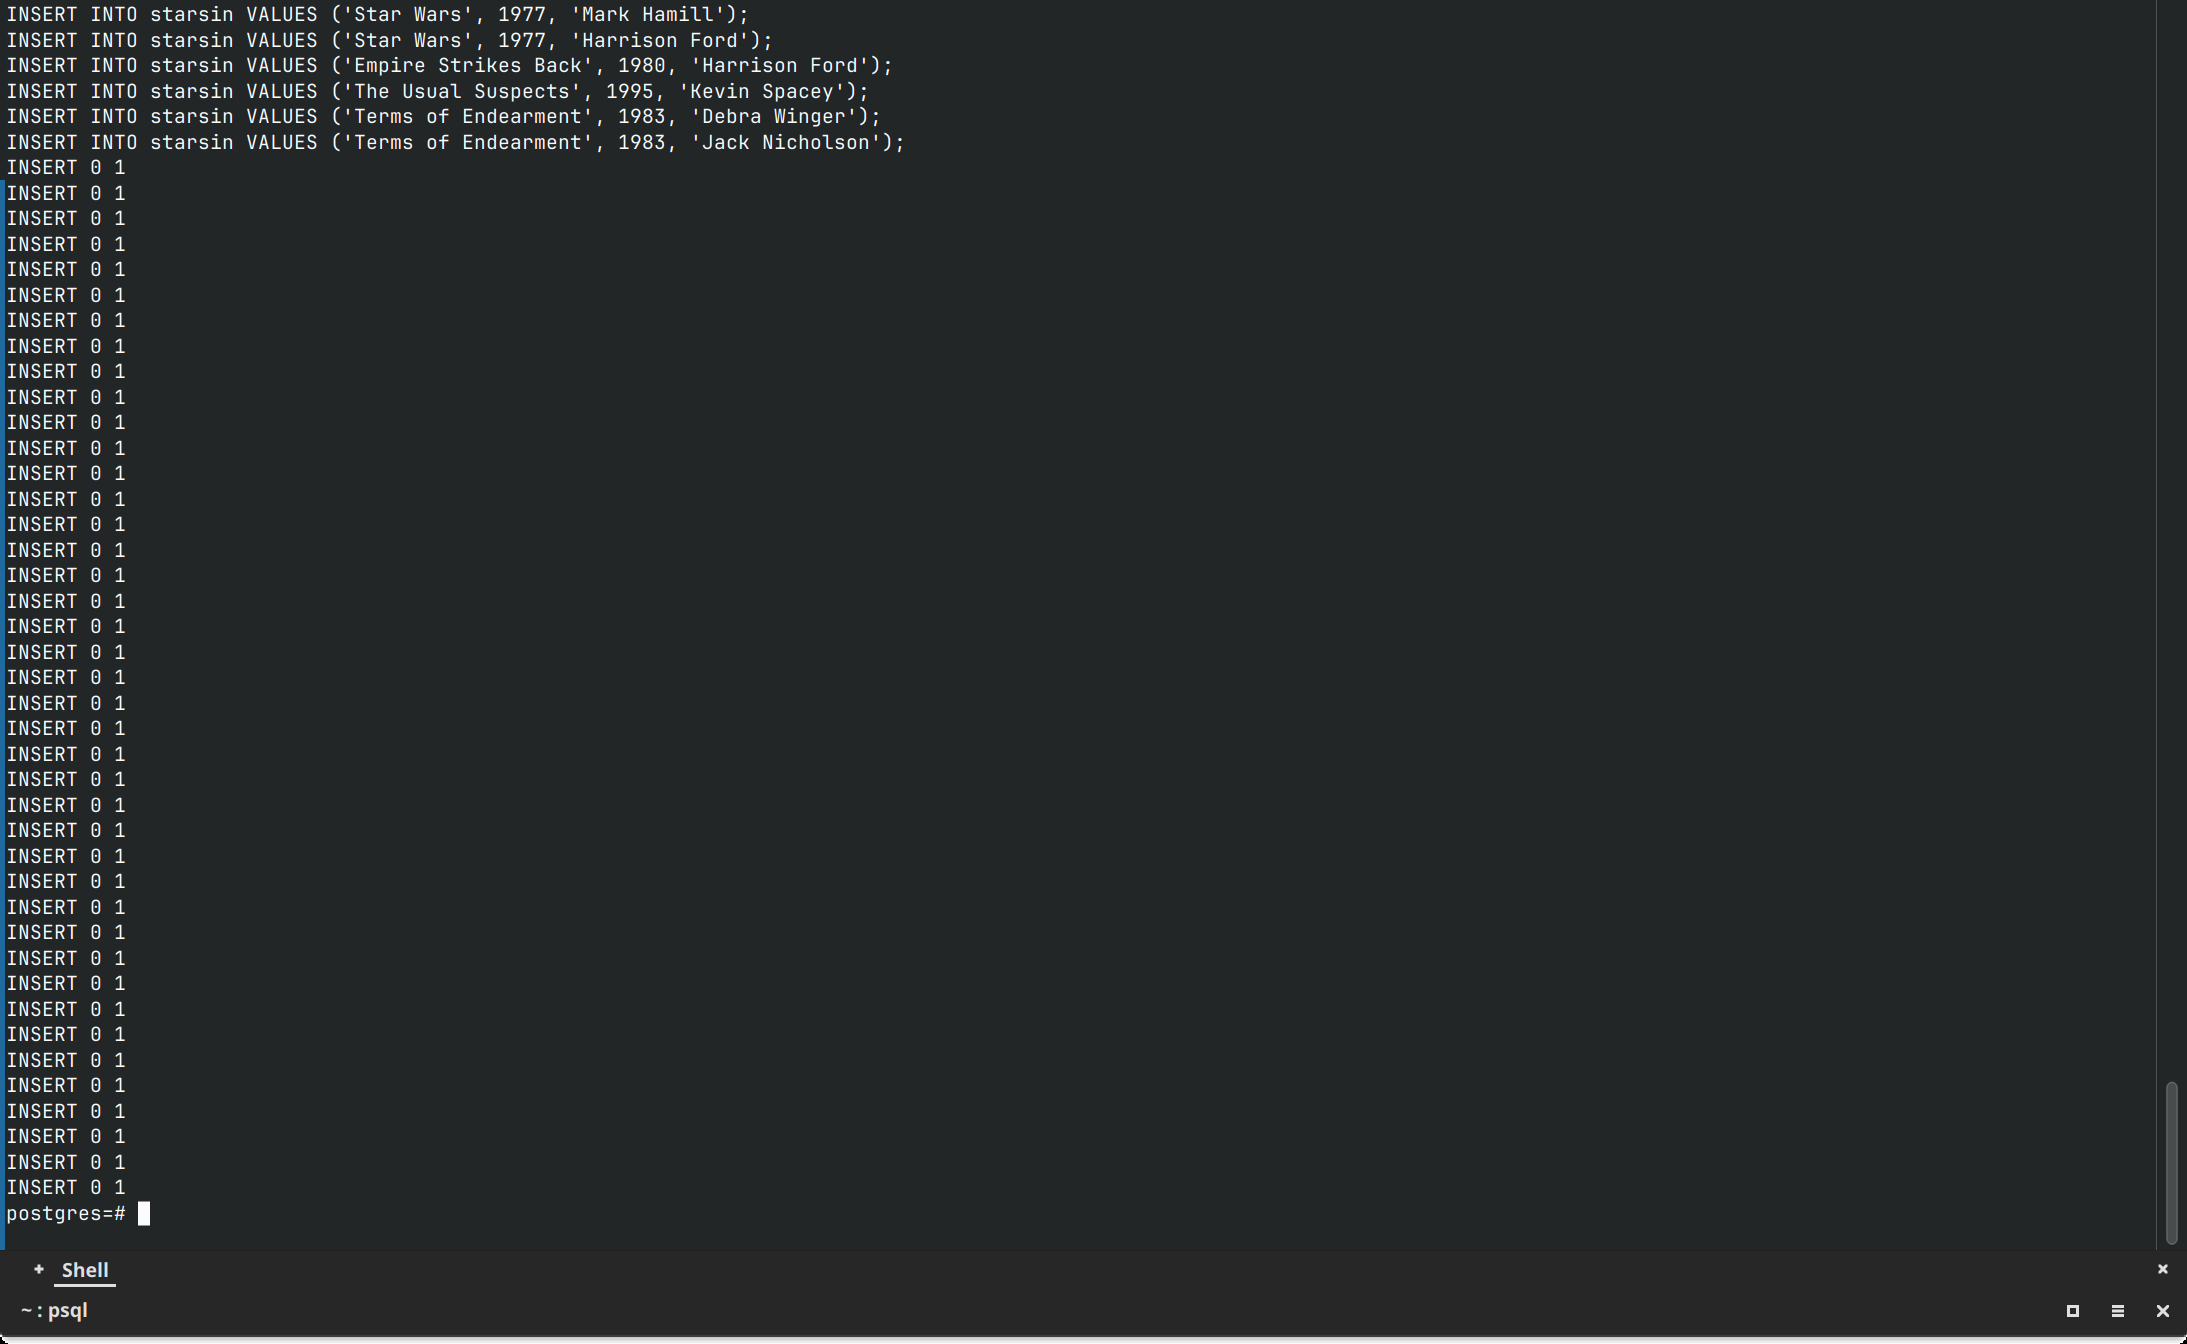
\includegraphics[width=0.9\textwidth]{hw4-10.png}
    \caption{Queries on More Than One Table Results}
    \label{fig:more-than-one-table-2}
\end{figure}

\subsubsection{Products Query}

\begin{lstlisting}
SELECT moviestar.name, movieexec.name
FROM moviestar,
        movieexec
WHERE moviestar.address = movieexec.address;

SELECT Star1.name, Star2.name
FROM moviestar Star1,
        moviestar Star2
WHERE Star1.address = Star2.address
    and Star1.name < Star2.name;
\end{lstlisting}

the execute results is shown in Figure \ref{fig:products-query}.

\begin{figure}[htbp]
    \centering
    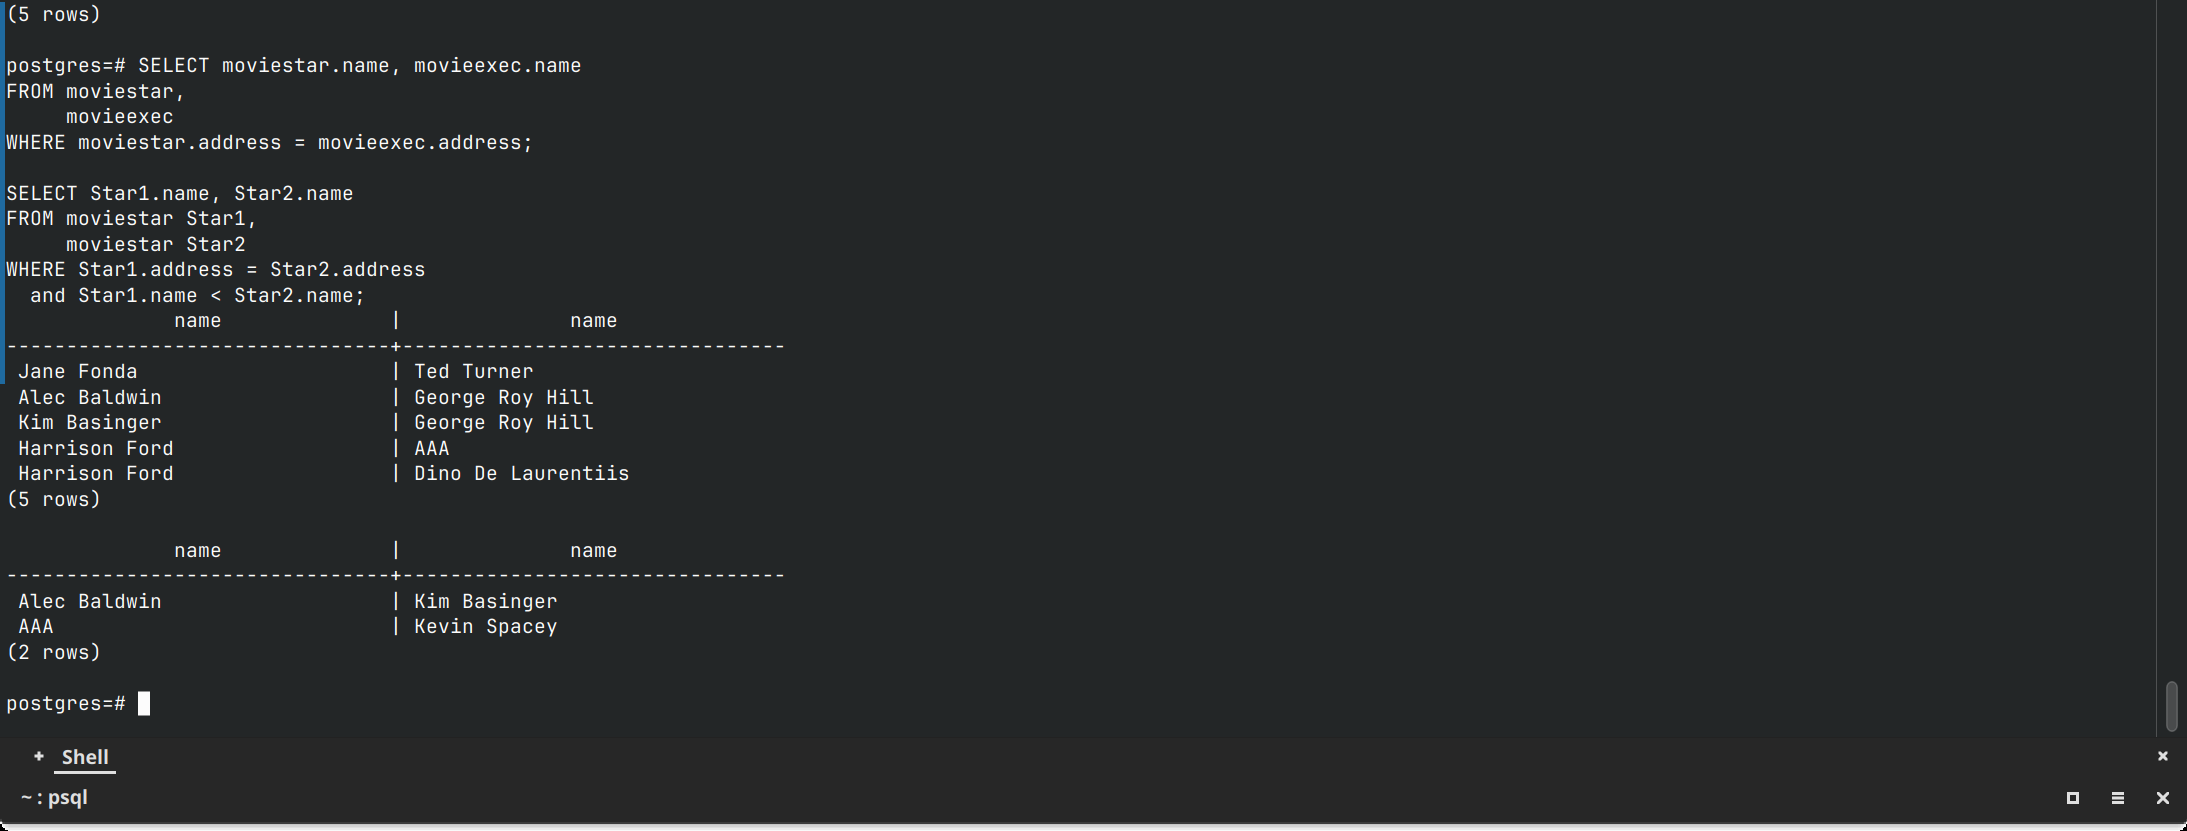
\includegraphics[width=0.9\textwidth]{hw4-11.png}
    \caption{Queries on More Than One Table Results}
    \label{fig:products-query}
\end{figure}

\subsubsection{Union, Intersection and Difference}

\begin{lstlisting}          
(SELECT name, address
 FROM MovieStar
 WHERE gender = 'F')
INTERSECT
(SELECT name, address
 FROM MovieExec
 WHERE netWorth > 10000000);

(SELECT name, address FROM MovieStar)
EXCEPT
(SELECT name, address FROM MovieExec);

(SELECT title, year FROM Movies)
UNION
(SELECT movieTitle AS title, movieYear AS year FROM StarsIn);
\end{lstlisting}

the execute results is shown in Figure \ref{fig:union-intersection-difference}.
\begin{figure}[htbp]
    \centering
    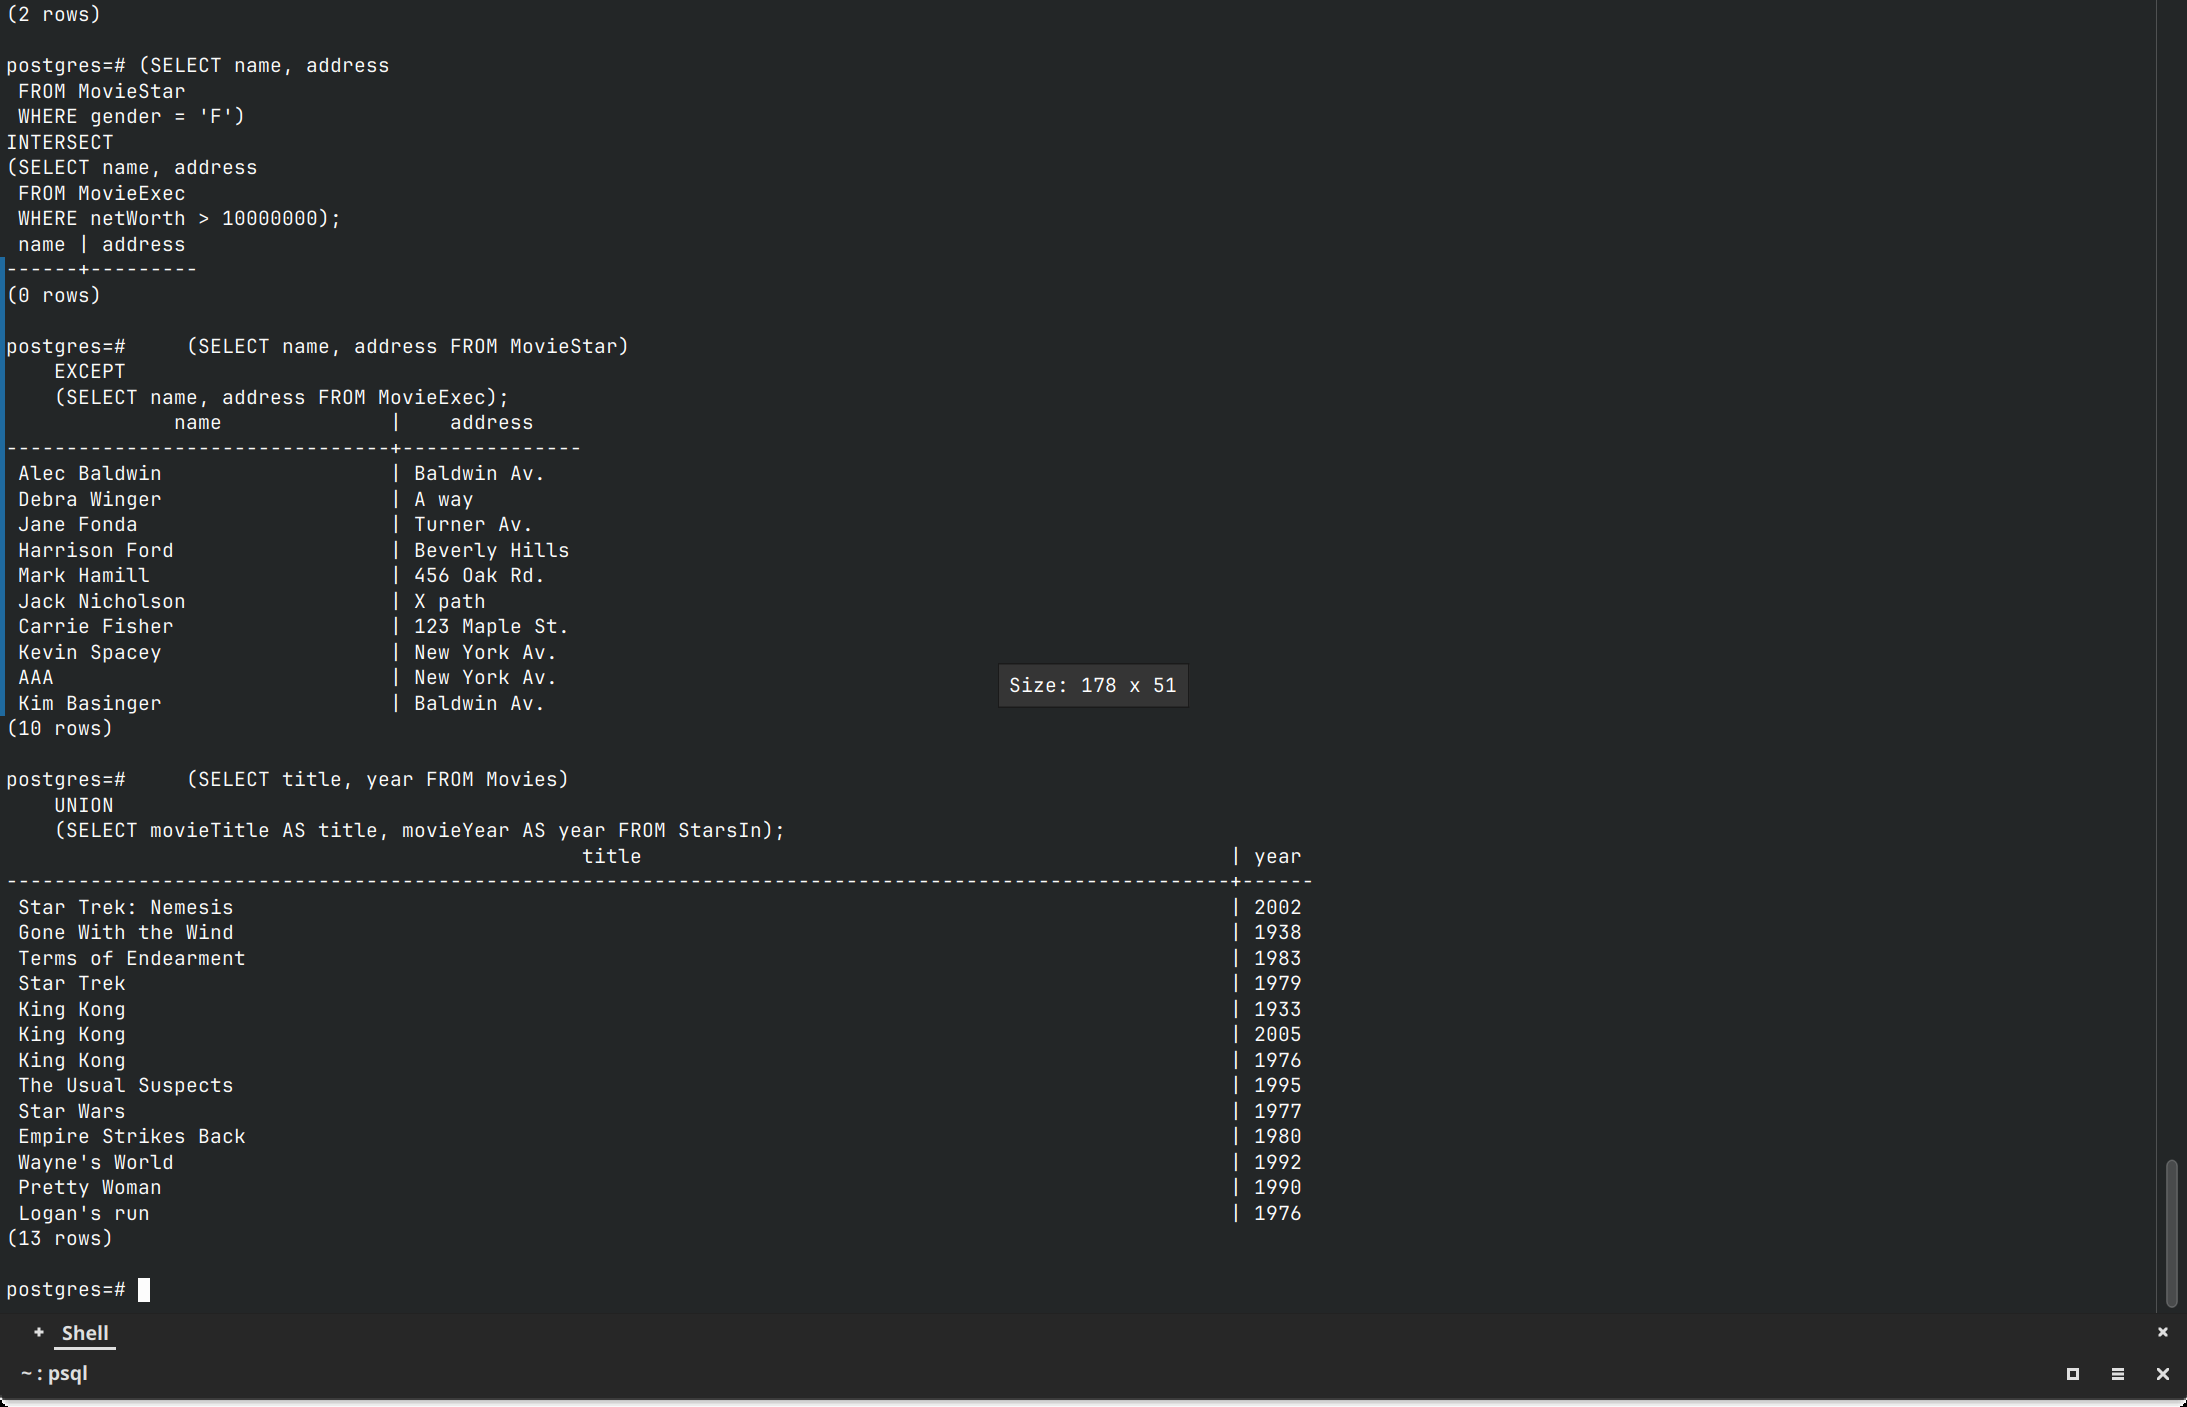
\includegraphics[width=0.9\textwidth]{hw4-12.png}
    \caption{Union, Intersection and Difference Results}
    \label{fig:union-intersection-difference}
\end{figure}

\section{Exercise 6.1.4 }
\textbf{Exercise 6.1.4:} Write the following queries based on the database schema of Exercise 2.4.3:

\begin{itemize}
    \item \texttt{Classes(class, type, country, numGuns, bore, displacement)}
    \item \texttt{Ships(name, class, launched)}
    \item \texttt{Battles(name, date)}
    \item \texttt{Outcomes(ship, battle, result)}
\end{itemize}

and show the result of your query on the data of Exercise 2.4.3.

\begin{enumerate}
    \item[a)] Find the class name and country for all classes with at least 10 guns.
    \item[b)] Find the names of all ships launched prior to 1918, but call the resulting column \texttt{shipName}.
    \item[c)] Find the names of ships sunk in battle and the name of the battle in which they were sunk.
    \item[d)] Find all ships that have the same name as their class.
    \item[e)] Find the names of all ships that begin with the letter ``R.''
    \item[f)] Find the names of all ships whose name consists of three or more words (e.g., \textit{King George V}).
\end{enumerate}

\subsection{Solutions}

\subsubsection*{a. Find the class name and country for all classes with at least 10 guns.}

\begin{lstlisting}
SELECT class, country FROM Classes WHERE numGuns >= 10;
\end{lstlisting}

\subsubsection*{b. Find the names of all ships launched prior to 1918, but call the resulting column \texttt{shipName}.}

\begin{lstlisting}
SELECT name AS shipName FROM Ships WHERE launched < 1918;
\end{lstlisting}

\subsubsection*{c. Find the names of ships sunk in battle and the name of the battle in which they were sunk.}

\begin{lstlisting}
SELECT ship, battle FROM Outcomes WHERE result = 'sunk';
\end{lstlisting}

\subsubsection*{d. Find all ships that have the same name as their class.}

\begin{lstlisting}
SELECT Ships.name FROM Ships, Classes WHERE Ships.class = Classes.class;

-- or using join keywords
SELECT Ships.name FROM Ships
JOIN Classes ON Ships.class = Classes.class;
\end{lstlisting}

\subsubsection*{e. Find the names of all ships that begin with the letter \texttt{R}}

\begin{lstlisting}
SELECT name FROM Ships WHERE name LIKE 'R%';
\end{lstlisting}

\subsubsection*{f. Find the names of all ships whose name consists of three or more words (e.g., \textit{King George V}).}

\begin{lstlisting}
SELECT name FROM Ships WHERE name LIKE '% % %';
\end{lstlisting}

\section{Exercise 6.2.1}
\textbf{Exercise 6.2.1:} Using the database schema of our running movie example

\begin{itemize}
    \item \texttt{Movies(title, year, length, genre, studioName, producerC\#)}
    \item \texttt{StarsIn(movieTitle, movieYear, starName)}
    \item \texttt{MovieStar(name, address, gender, birthdate)}
    \item \texttt{MovieExec(name, address, cert\#, netWorth)}
    \item \texttt{Studio(name, address, presC\#)}
\end{itemize}

write the following queries in SQL.

\begin{enumerate}
    \item[a)] Who were the male stars in \textit{Titanic}?
    \item[b)] Which stars appeared in movies produced by MGM in 1995?
    \item[c)] Who is the president of MGM studios?
    \item[d)] Which movies are longer than \textit{Gone With the Wind}?
    \item[e)] Which executives are worth more than Merv Griffin?
\end{enumerate}

\subsection{Solutions}

\subsubsection*{a. Who were the male stars in \textit{Titanic}?}

\begin{lstlisting}
SELECT starName FROM starsin WHERE movieTitle='Titanic' AND starName IN (SELECT name FROM moviestar WHERE gender='M');

-- or using join keywords
SELECT starName FROM starsin
JOIN moviestar ON starsin.starName = moviestar.name
WHERE movieTitle='Titanic' AND gender='M';
\end{lstlisting}

\subsubsection*{b. Which stars appeared in movies produced by MGM in 1995?}

\begin{lstlisting}
-- Using subquery
SELECT starName FROM starsin
WHERE (movieTitle, movieYear) IN (
    SELECT title, year FROM movies WHERE studioName = 'MGM' AND year = 1995
);

-- Using join keywords
SELECT starName FROM starsin
JOIN movies ON starsin.movieTitle = movies.title AND starsin.movieYear = movies.year
WHERE movies.studioName = 'MGM' AND movies.year = 1995;
    
\end{lstlisting}

\subsubsection*{c. Who is the president of MGM studios?}

\begin{lstlisting}
-- Using subquery
SELECT name FROM movieexec
WHERE "cert#" = (SELECT "presC#" FROM studio WHERE name = 'MGM');

-- Using JOIN
SELECT movieexec.name FROM movieexec
JOIN studio ON movieexec.cert# = studio.presC#
WHERE studio.name = 'MGM';
    
\end{lstlisting}

\subsubsection*{d. Which movies are longer than \textit{Gone With the Wind}?}

\begin{lstlisting}
-- Ensure uniqueness by specifying the year if known
SELECT title FROM movies WHERE length > (
    SELECT length FROM movies WHERE title = 'Gone With the Wind'
);

-- Corrected JOIN version
SELECT movies.title FROM movies
JOIN movies GWTW ON GWTW.title = 'Gone With the Wind'
WHERE movies.length > GWTW.length;
    
\end{lstlisting}

\subsubsection*{e. Which executives are worth more than Merv Griffin?}

\begin{lstlisting}
SELECT name FROM movieexec WHERE netWorth > (SELECT netWorth FROM movieexec WHERE name='Merv Griffin');

-- or using join keywords
SELECT movieexec.name FROM movieexec
JOIN movieexec MG ON MG.name = 'Merv Griffin'
WHERE movieexec.netWorth > MG.netWorth;
\end{lstlisting}



\end{document}
